\begin{minipage}{0.60\textwidth}
    \begin{figure}[h]
    \centering
    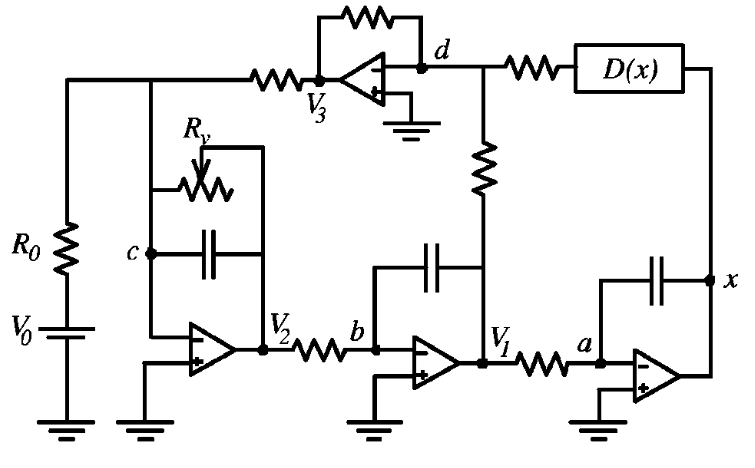
\includegraphics[width=1\textwidth]{images/e_chaotic_circuit.png}
    \caption{Schematic diagram of the circuit used.}
    %\label{fig:}
\end{figure}
\end{minipage}
\hfill
\begin{minipage}{0.35\textwidth}
    \begin{figure}[h]
        \centering
        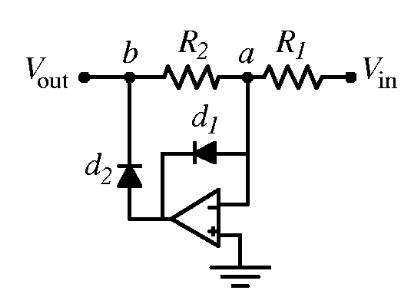
\includegraphics[width=1\textwidth]{images/e_nonlinear_elements.png}
        \caption{Nonlinear subcircuit D(x). $V_{\text{out}} = D (V_{\text(in)}) = -(R_2/R_1)\text{min}(V_{\text{in}}, 0)$.}
        %\label{fig:}
    \end{figure}
    
\end{minipage}
\begin{equation}
    R C \frac{d V_2}{d t} = - \left(\frac{R}{R_v}\right)V_2 - \left(\frac{R}{R_0}\right)V_0 - V_3.
\end{equation}